\documentclass{article}
\usepackage{tikz}

\begin{document}

\begin{figure}[h]
    \centering
    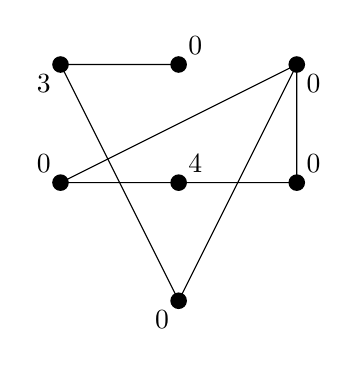
\begin{tikzpicture}[scale=1.5]
        % Define coordinates
        \coordinate (A) at (0,0);
        \coordinate (B) at (1,0);
        \coordinate (C) at (2,0);
        \coordinate (D) at (1,1);
        \coordinate (E) at (0,1);
        \coordinate (F) at (2,1);
        \coordinate (G) at (1,-1);
        
        % Draw edges
        \draw (A) -- (B) -- (C) -- (F) -- cycle;
        \draw (D) -- (E) -- (G) -- (F);
        
        % Draw nodes with labels
        \fill (A) circle (2pt) node[above left] {0};
        \fill (B) circle (2pt) node[above right] {4};
        \fill (C) circle (2pt) node[above right] {0};
        \fill (D) circle (2pt) node[above right] {0};
        \fill (E) circle (2pt) node[below left] {3};
        \fill (F) circle (2pt) node[below right] {0};
        \fill (G) circle (2pt) node[below left] {0};
    \end{tikzpicture}
    \caption{The condition $g(\Gamma) \geq 5$ is necessary in Proposition \ref{cota2}.}
\end{figure}

\end{document}